% --------------------------------------------------------------
% This is all preamble stuff that you don't have to worry about.
% Head down to where it says "Start here"
% --------------------------------------------------------------
 
\documentclass[12pt]{article}

\usepackage{courier}
\usepackage{color}
\usepackage{listings}
\usepackage[square,numbers]{natbib}
\usepackage{tabls}
\usepackage{graphicx}
\usepackage{subcaption}
\usepackage{pdfpages}
\usepackage{mathtools}

\definecolor{dkgreen}{rgb}{0,0.6,0}
\definecolor{gray}{rgb}{0.5,0.5,0.5}




\lstset{language=python,
   basicstyle=\ttfamily,
   keywordstyle=\color{blue},
   commentstyle=\color{dkgreen},
   stringstyle=\color{red},
   numbers=left,
   numberstyle=\tiny\color{gray},
   stepnumber=1,
   numbersep=10pt,
   backgroundcolor=\color{white},
   tabsize=4,
   showspaces=false,
   showstringspaces=false}
 
\usepackage[margin=1in]{geometry} 
\usepackage{amsmath,amsthm,amssymb}
\usepackage{verbatim}
\usepackage{algpseudocode,algorithm}
\usepackage{setspace}

\newcommand{\ihat}{\ensuremath{\hat{\textbf{\i}}}}
\newcommand{\keff}{\ensuremath{k_{\mathrm{eff}}}}
\newcommand{\jhat}{\ensuremath{\hat{\textbf{\j}}}}
\newcommand{\lline}{\noindent\makebox[\linewidth]{\rule{\textwidth}{0.4pt}}}
\newcommand{\N}{\mathbb{N}}
\newcommand{\Z}{\mathbb{Z}}
\newcommand{\deriv}[2]{\frac{\mathrm{d} #1}{\mathrm{d} #2}}
\newcommand{\pderiv}[2]{\frac{\partial #1}{\partial #2}}
\newcommand{\bx}{\mathbf{X}}
\newcommand{\ba}{\mathbf{A}}
\renewcommand{\d}{\mathrm{d}}
\newcommand{\A}{\frac{(1-\alpha)}{2(1+\alpha)}}
\newcommand{\upl}{u_{\text{plane}}}
\newcommand{\upt}{u_{\text{point}}}
\newcommand{\D}{\Delta}
\newcommand{\ra}{\rightarrow}
\renewcommand{\SS}{\State}
 
\newenvironment{theorem}[2][Theorem]{\begin{trivlist}
\item[\hskip \labelsep {\bfseries #1}\hskip \labelsep {\bfseries #2.}]}{\end{trivlist}}
\newenvironment{lemma}[2][Lemma]{\begin{trivlist}
\item[\hskip \labelsep {\bfseries #1}\hskip \labelsep {\bfseries #2.}]}{\end{trivlist}}
\newenvironment{exercise}[2][Exercise]{\begin{trivlist}
\item[\hskip \labelsep {\bfseries #1}\hskip \labelsep {\bfseries #2.}]}{\end{trivlist}}
\newenvironment{problem}[2][Problem]{\begin{trivlist}
\item[\hskip \labelsep {\bfseries #1}\hskip \labelsep {\bfseries #2:}]\hspace{0.3in}\newline\newline}{\end{trivlist}}
\newenvironment{question}[2][Question]{\begin{trivlist}
\item[\hskip \labelsep {\bfseries #1}\hskip \labelsep {\bfseries #2.}]}{\end{trivlist}}
\newenvironment{corollary}[2][Corollary]{\begin{trivlist}
\item[\hskip \labelsep {\bfseries #1}\hskip \labelsep {\bfseries #2.} ]}{\end{trivlist}}
\newenvironment{problem*}[1][Problem]{\begin{trivlist}
\item[\hskip \labelsep {\bfseries #1} {\hspace{-0.2em}\bfseries:}]}{\end{trivlist}}
\newenvironment{solution}[1][Solution]{\begin{trivlist}
\item[\hskip \labelsep {\bfseries #1} {\hspace{-0.2em}\bfseries:}]\hspace{0.3in}\newline}{\end{trivlist}}
\newenvironment{solnum}[2][Solution]{\begin{trivlist}
\item[\hskip \labelsep {\bfseries #1}\hskip \labelsep {\bfseries #2:}]\hspace{0.3in}\newline\newline}{\end{trivlist}}
\newcommand{\iso}[2]{\ensuremath{^{#2}\text{#1}}}
\newcommand{\nubar}{\ensuremath{\overline{\nu}}}
 
\begin{document}
 
% --------------------------------------------------------------
%                         Start here
% --------------------------------------------------------------
 
\title{Homework 3}%replace X with the appropriate number
\author{Simon Bolding\\ %replace with your name
NUEN 629} %if necessary, replace with your course title
 
\maketitle

\clearpage

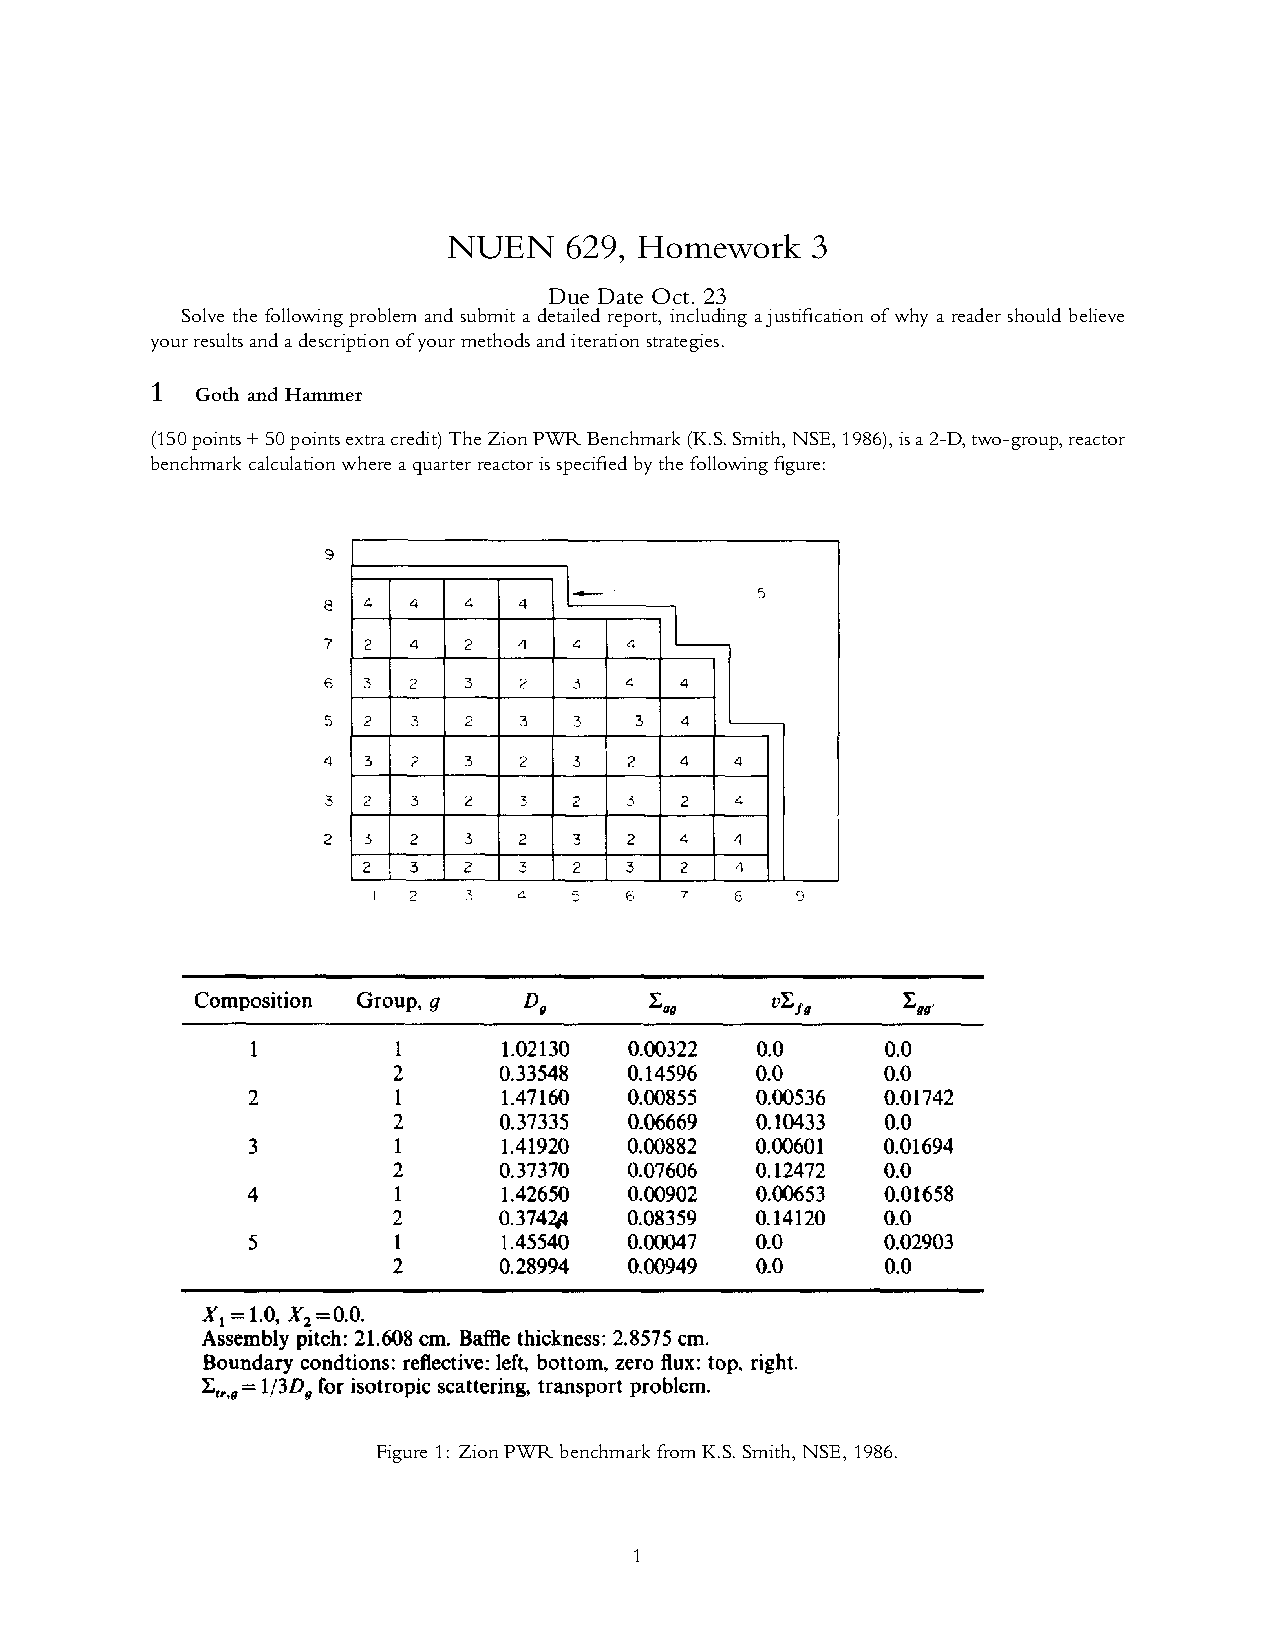
\includepdf{Homework3.pdf}

\begin{solnum}{1-1}
    
The 2D lattice input code provided in lab was modified to generate an input for zion
benchmark problem.  Because the
provided code assumes a uniform mesh size, approximations must be made to resolve the
baffle in the geometry.  I have assumed that if a particular cells center lies with
in the region of the baffle, then that cell has the baffle material properties.  Also, I have assumed that the assemblies near the reflecting
boundary are full assemblies, rather than half assemblies.

\end{solnum}

\begin{solnum}{1-2}

The provided algorithms for the nodal method in class had to be modified. Although it
is not the most efficient, we have modified.

\begin{solnum}{1-3}

Because the nodal code is very slow, the finite difference code was used to determine
the critical reactor height. The secant method was used to determine the critical
height to 4 digits of accuracy.  The critical height was found to be BLARG cm. This
is a reasonable number since the 2D reactor had a relatively high $\keff$ of
$\sim$1.27.
\end{solnum}

\clearpage

\begin{solnum}{2}

First, we need an atom density of the hydrogen.  Based on ideal gas law, the density
scales proportional to tempurature.  At 1 atm, the density of hydrogen at room
temperature is roughly 9.E-04 g cm$^{-3}$.  Scaling by 30, gives a density of 0.0025
g cm$^{-3}$.  This is in agreement to 1 significant digit with an online calculator that takes into account
compressibility of hydrogen at 30 atm and room temperature.  This gives a
corresponding atom density of hydrogen as
\begin{equation}
    N^{H} = 0.0025 \frac{\text{g}}{\text{cm}^3}\frac{1\text{ mol H}_2}{2.02\text {g
    H}_2}\frac{2 H}{1 H_2}\frac{0.60221\text{ atoms cm}^2}{\text{b}} \approx
    0.00149\;\frac{\text{H atoms}}{\text{b--cm}}
\end{equation}

As an initial approximation, I assumed that within the semi-infinite Hydrogen medium, several
mfp away from the source, the sphere of \iso{U}{235} will appear as an isotropic
boundary source to a 1D, semi-infinite medium.  Following the notes, the general multigroup
1D transport equation we will be solving, in the Hydrogen, will have the form
\begin{equation}\label{te_orig}
    \mu\pderiv{\psi_g(z,\mu)}{z} +\hat\Sigma_{tg}\psi_g = \sum_{l=0}^\infty
    \frac{2l+1}{2} P_l(\mu) \sum_{g'=0}^{G-1}\left[\Sigma_{slg'\ra g} +
    \delta_{gg'}\left(\hat\Sigma_{tg'}-\Sigma_{tlg'}\right)\right]\phi_{lg'}(z) +
    q(\mu,z),
\end{equation}
where $\hat\Sigma_{tg}$ is yet to be defined.
Also, it is assumed that the spectrum of energies leaving the sphere of \iso{U}{235} is well
approximated by the fission emission energy spectrum $\chi(E)$ (i.e., only consider the
uncollided energy spectrum).  The group integrated $\chi(E)$ for \iso{U}{235} is
computed.  All groups have a high scattering ratio of $\approx0.9999$.  Thus, a
few MFP away from the boundary source, we expect diffusion theory to be applicable,
with essentially a pure scatter. Consider the 1-speed diffusion theory equation for a pure
scatterer, in a semi-infinite medium, with no internal source
\begin{equation}
    -D \frac{\d^2\phi}{\d x^2} = 0.
\end{equation}
The requirement that the flux be bounded at infinity requires a constant spatial
solution, so we thus can neglect spatial gradients in Eq.~\eqref{te_orig}.
We choose to normalize the effective source of neutrons from the sphere such that the
magnitude of the energy integrated source is 1.  Thus, our transport equation to be solved becomes
\begin{equation}
    \hat\Sigma_{t,g}\psi_g(\mu) = \sum_{l=0}^\infty
    \frac{2l+1}{2} P_l(\mu) \sum_{g'=0}^{G-1}\left[\Sigma^*_{slg'\ra g} +
    \delta_{gg'}\left(\hat\Sigma_{tg'}-\Sigma_{tlg'}\right)\right]\phi_{lg'} +
    \frac{\chi_g}{2}
\end{equation}
where the $\Sigma_s^*$ will depend on the method.
Taking the zeroth moment gives the equation for the scalar flux in each group as
\begin{equation}
    \hat\Sigma_{t,g}\phi_g = \sum_{g'=0}^{G-1}\left[\Sigma_{s0g'\ra g} +
    \delta_{gg'}\left(\hat\Sigma_{tg'}-\Sigma_{t0g'}\right)\right]\phi_{g'} +
    \chi_g
\end{equation}
The first moment gives the equation for the current in each group as
\begin{equation}
    \hat\Sigma_{t,g}J_g = \sum_{g'=0}^{G-1}\left[\Sigma_{s1g'\ra g} +
    \delta_{gg'}\left(\hat\Sigma_{tg'}-\Sigma_{t1g}\right)\right]J_g'.
\end{equation}
The only solution to the above equation is 0.  So, based on our assumptions of an
isotropic source, for all methods and all groups, $\boxed{J_g=0}$.

The equation for the scalar flux can be written as a matrix equation as
\begin{equation}
    \mathbf{S\Phi} = \boldsymbol{\chi}
\end{equation}
with matrix elements defined as
\begin{equation}
    \chi_i = \chi_{g_i}, \quad g_i=0,1,\ldots,G-1
\end{equation}
\begin{equation}
    \phi_i = \phi_{g_i}, \quad g_i=0,1,\ldots,G-1
\end{equation}
and
\begin{equation}
    S_{ij} = \left\{\begin{matrix}
        \hat\Sigma_{t,g_i} -\Sigma^*_{s0g_{i}\ra g_{i}} & i=j
        \\  
        -\Sigma^*_{s0g_i\ra g_j} & i \neq j
    \end{matrix}\right.
\end{equation}

For the approximation of separable in energy, the effective cross sections become $\hat\Sigma_{t,g} = \Sigma_{t,g}$ and
$\Sigma^*_{s0,g'\ra g} = \Sigma_{s0,g'\ra g}$.
For the P$_1$ consistent form of the equation, we set $\hat\Sigma_{t,g} =
\Sigma_{t0,g}$, which gives the same equations for scalar flux since we
are only interested in the $0$-th moment cross sections. For the extended Legendre
expansion we want
\begin{equation}
    \hat\Sigma_{tg} = \Sigma_{t,L+1,g} - \sum_{g'=0}^{G-1} \Sigma_{s,L+1,g\ra g'}
\end{equation}
where since we are interested in the scalar flux we will choose $L=0$, giving
\begin{equation}
    \hat\Sigma_{tg} = \Sigma_{t1,g} - \sum_{g'=0}^{G-1} \Sigma_{s1,g\ra g'}
\end{equation}
If we make the approximation
\begin{equation}
\Sigma_{t1,g} \approx \Sigma_{s1,g} := \sum_{g'=0}^{G-1} \Sigma_{s1,g\ra g'}
\end{equation}
then we get $\hat\Sigma_{tg} = 0$.  This leads to an identical set of equations as
the other two methods.

Solving the matrix system gives a solution for $\phi_g$ (the same for all three
methods).  A plot of the solutions
in each group are compared below. The code is given at the end of the assignment

\begin{figure}[h!]
    \centering
    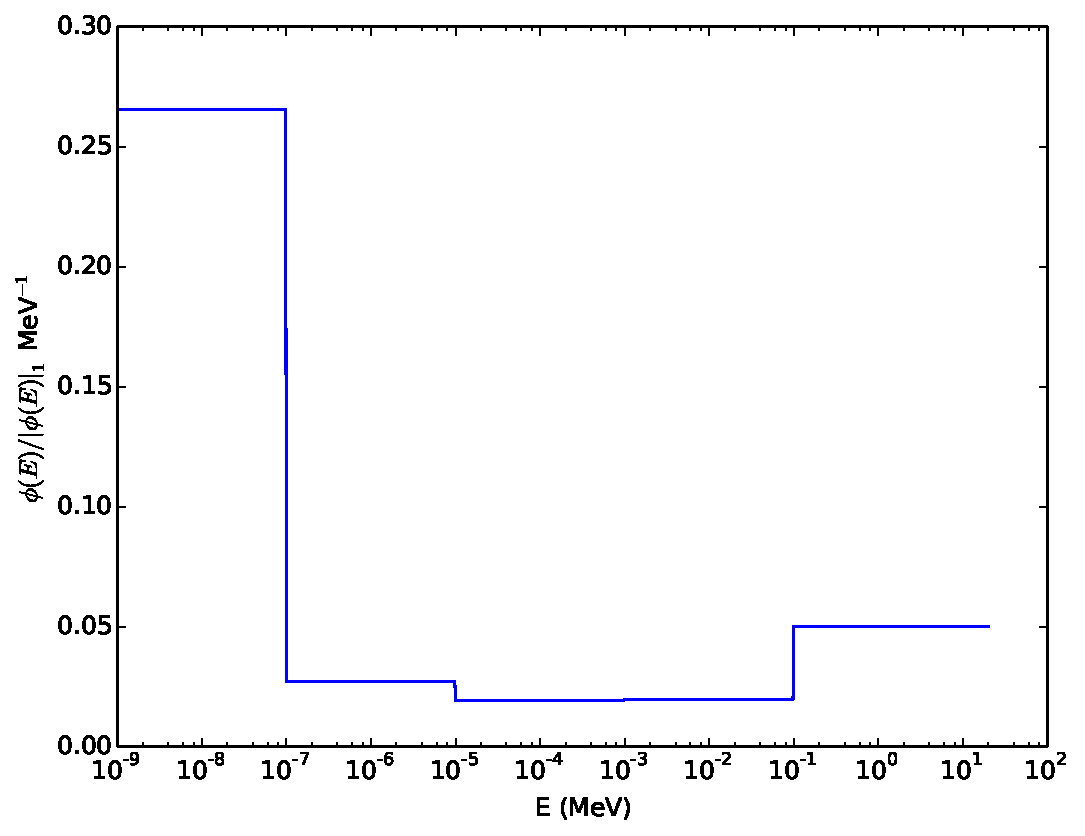
\includegraphics[width=0.5\textwidth]{method_compare.pdf}
\end{figure}





    



\end{solnum}


%\includepdf[pages={1}]{p1p3.pdf}
\clearpage
    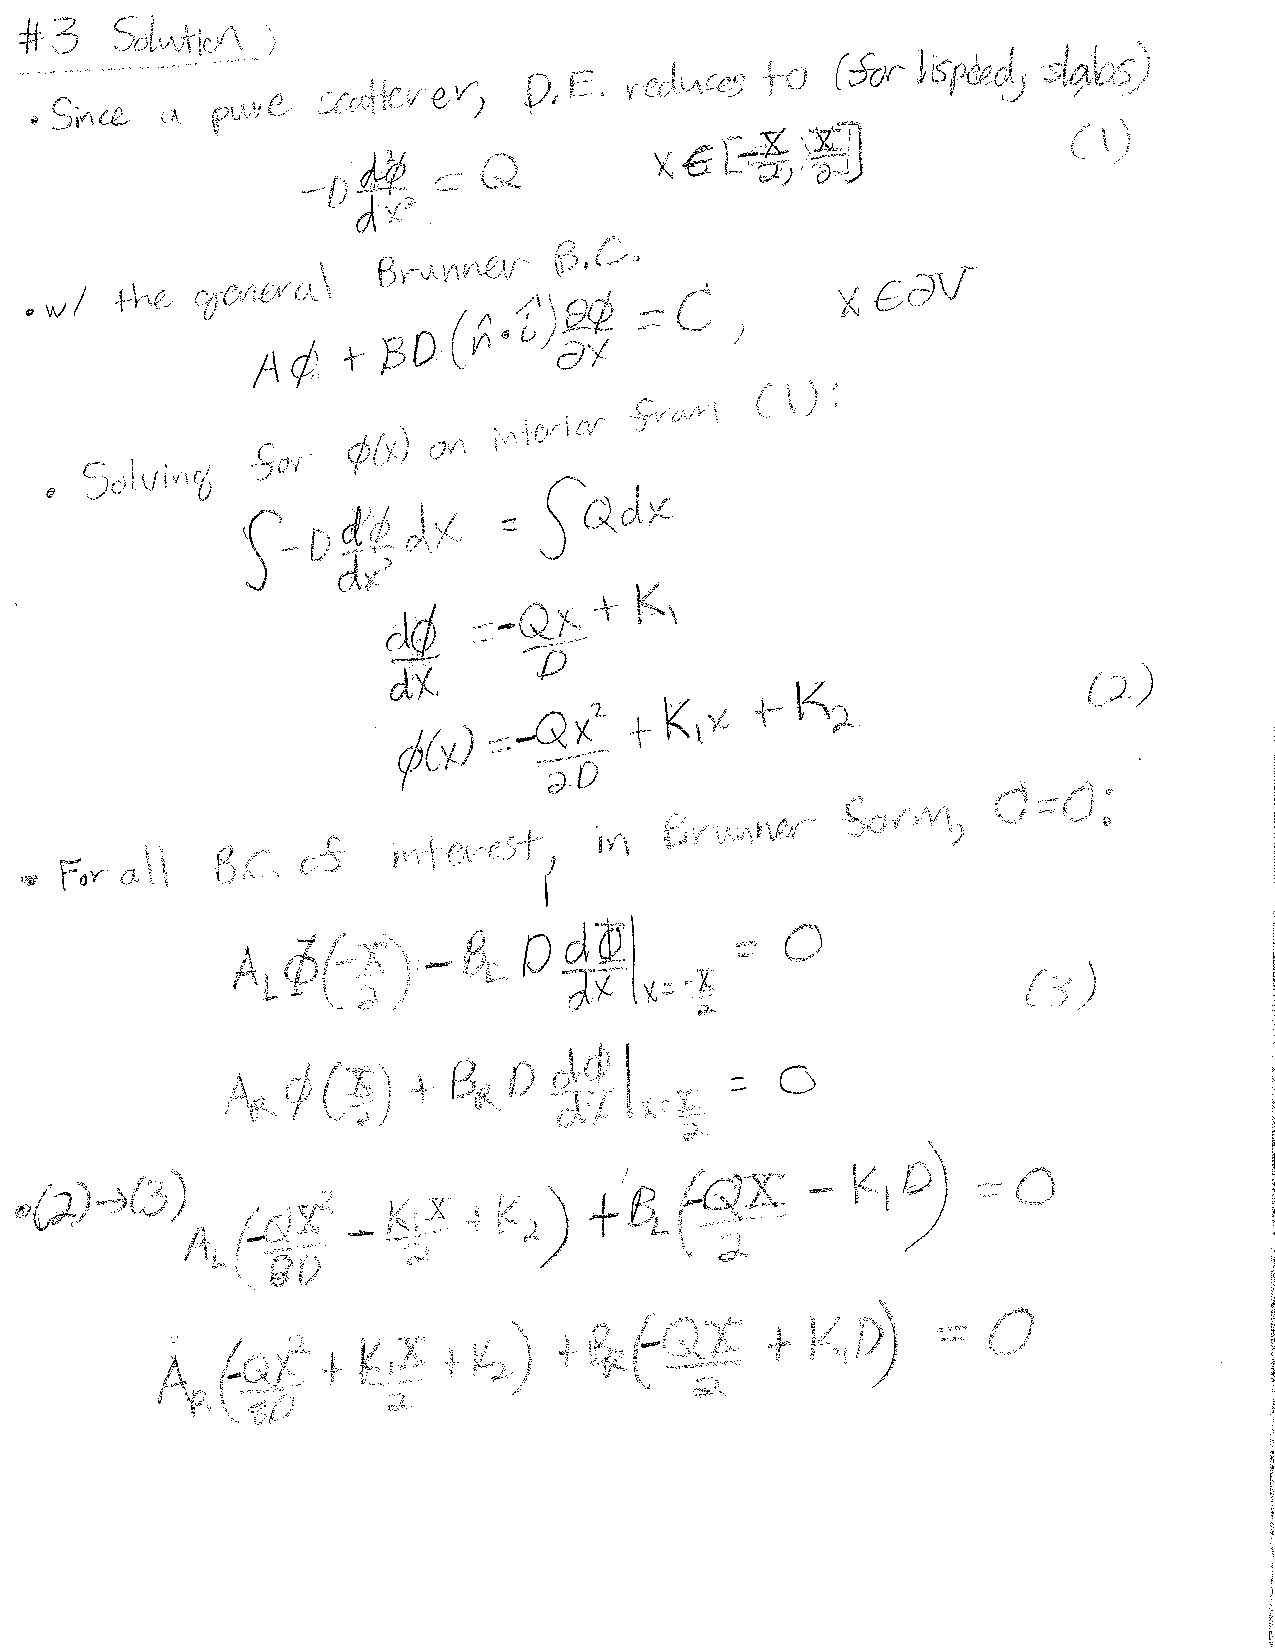
\includepdf[pages={1-2}]{p3.pdf}
    A summary of the solutions obtained for each of the boundary conditions is given
    in the table below. The figures below compares plots for the case of $Q=1$,
    $D=0.5$ and $X=10$.  The first figure demonstrates that Dirichlet (without use of
    the extrapolated BC) can be very inaccurate.  The solution with Mark boundary
    conditions is lower in magnitude than for the Marshak case, which is expected due
    to symmetry and that the Mark boundary condition has a shorter extrapolation
    distance of $\sqrt{3} D$, compared to $2D$ for Marshak. For the chosen parameters
    there is noticeable variation between the different choices of BC.  A smaller value of $D$ or increased $X$
    will result in more consistent solutions, particularly on the interior of the
    domain. The second plot shows that albedo varies between a Marshak and Reflective
    condition.  As expected, 
    reflective-type BC's on the right side of the domain results in a much larger magnitude in the solution
    as leakage is reduced but the source strength is the same as the vacuum cases.
    \begin{table}[h!]
        \centering
        \caption{Solutions with different boundary conditions for  a pure scatter for slab of width $X$ centered at
        $x=0$.}
        \begin{tabular}{|c|c|c|} \hline
            Left BC & Right BC & $\phi(x)$ \\ \hline
            Vac. Marshak & Vacuum Marshak & $\phi(x) = Q\left(\frac{X^2}{8D} + X-\frac{x^2}{2D} 
            \right)            $ \\ 
            Vac. Mark & Vacuum Marshak & $\phi(x) = Q\left(
            \frac{X^2}{8D} + \frac{X\sqrt{3}}{2}-\frac{x^2}{2D}\right)$ \\ 
            Vac. Dirichlet  & Vacuum Dirichlet & $\phi(x) = \frac{Q}{2D}\left( 
            \frac{X^2}{4} - x^2\right)  $ \\ 
            Vac. Dirichlet    & Albedo  & $\phi(x) = -\frac{Qx^2}{2D} +
            QxX\left(\frac{1+\A\frac{X}{2D}}{\A X + D} - \frac{1}{2D}  \right) +
            Q\frac{X^2}{2}\!\! \left(\frac{1+\A\frac{X}{2D}}{\A X +
            D}-\frac{1}{4D}\right) $ \\
            Vac. Dirichlet    & Reflecting & $\phi(x) =
            \frac{Q}{2D}\left(\frac{3X^2}{4} + xX  - {x^2}\right)$ \\ \hline
        \end{tabular}
    \end{table}
    \begin{figure}[h!]
        \centering
        \begin{subfigure}{0.495\textwidth}
            \centering 
            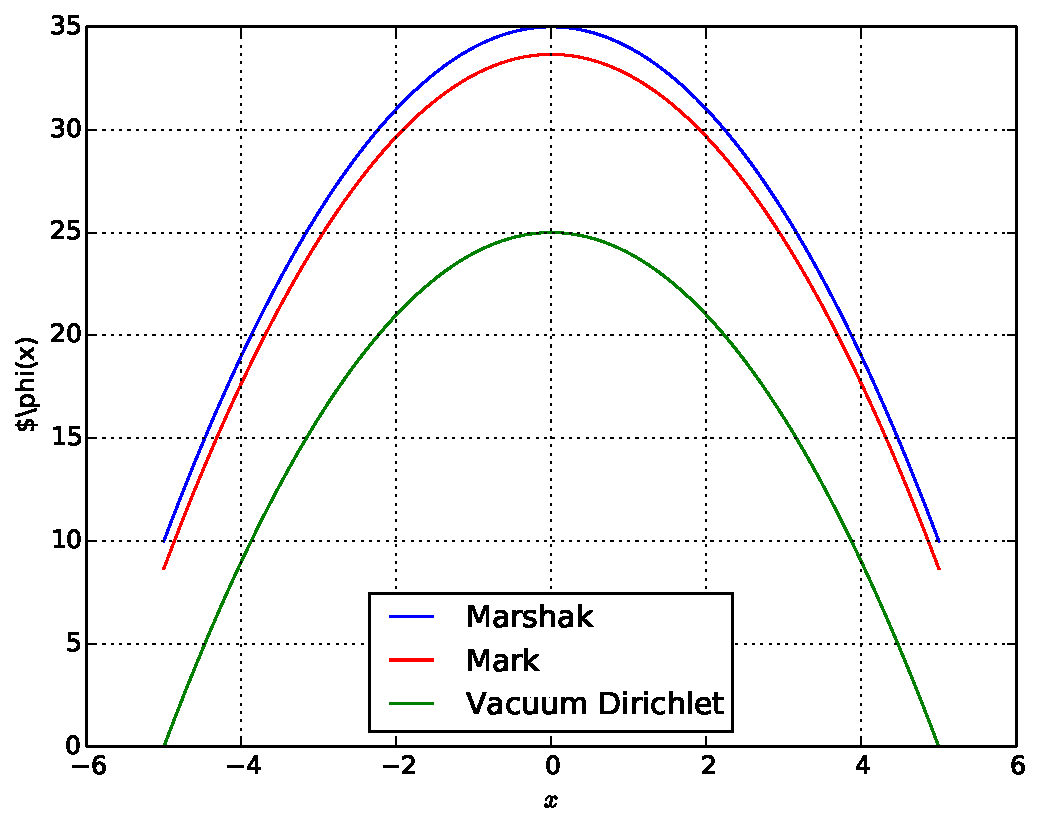
\includegraphics[width=0.99\textwidth]{diff_soln1.pdf}
        \end{subfigure}
        \begin{subfigure}{0.495\textwidth}
            \centering 
            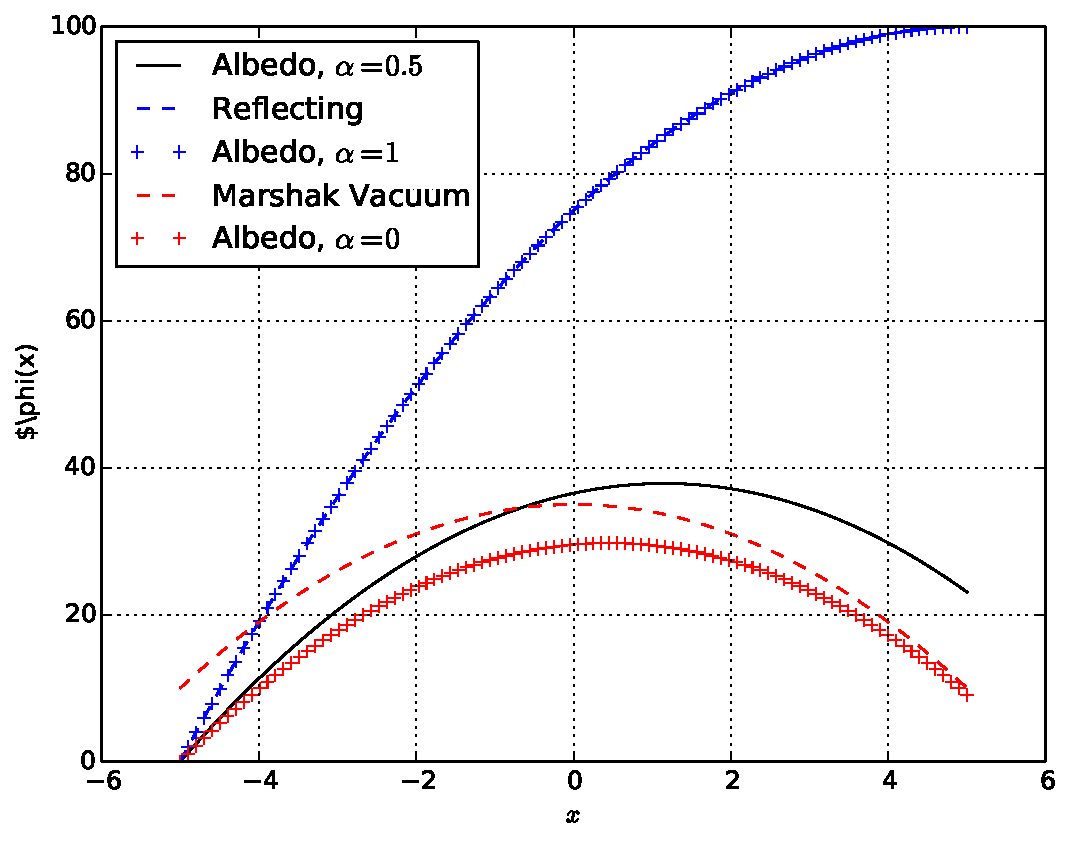
\includegraphics[width=0.99\textwidth]{diff_soln2.pdf}
        \end{subfigure}
        \caption{Comparison of Diffusion solutions for various boundary conditions
        with Q=1, D=0.5, X=10.}
    \end{figure}
\clearpage
\subsubsection*{Code for Problem 1}
\lstinputlisting[basicstyle=\scriptsize]{group_collapse/cxproc.py}
\lstinputlisting[basicstyle=\scriptsize]{energy_corrections/legendre.py}

\end{document}

